Neste capítulo é descrito como a aplicação proposta para a intervenção ao problema anteriormente evidenciado executa suas asções e como ocorre o fluxo de interações.

\section{Arquitetura da solução}

\begin{figure}[!htb]
        \caption{\label{diagrama1}Diagrama de Atividade}
        \begin{center}
                %\includegraphics[width=\textwidth, height=\textheight]{imagens/pretty.eps}
		%\includegraphics[width=0.5\textwidth, height=0.35\textheight]{imagens/teste.eps}
                \includegraphics[width=\textwidth]{imagens/teste.eps}
        \end{center}
        \legend{Fonte: Autor}
\end{figure}


\begin{figure}[!htb]
        \caption{\label{diagrama1}Fluxo de funcionamento da aplicação}
        \begin{center}
                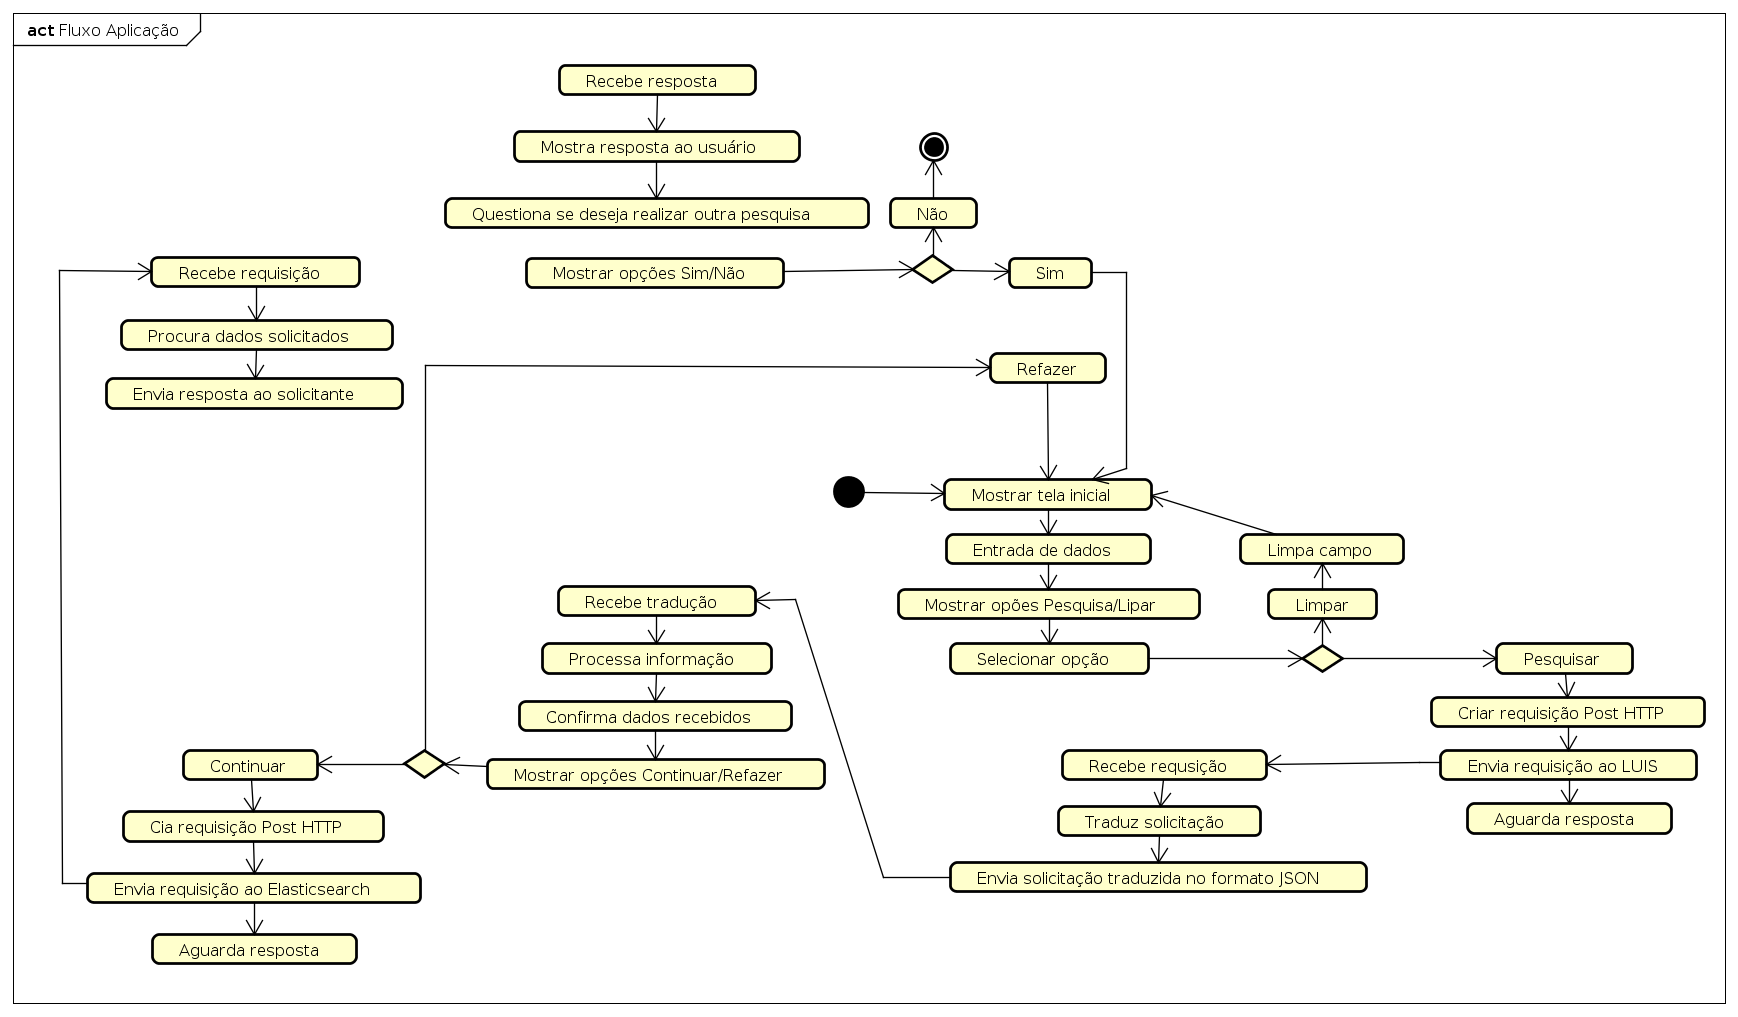
\includegraphics[angle=90, width=\textwidth, height=\textheight]{imagens/teste1.eps}
		%\includegraphics[width=0.5\textwidth, height=0.35\textheight]{imagens/teste.eps}
        \end{center}
        \legend{Fonte: Autor}
\end{figure}
